% !TeX spellcheck = de_DE
\section{Neuronale Netze}
Klassische Algorithmen in der Informatik beschreiben mit welchen Schritten ein spezielles Problem gelöst werden kann. In vielen Anwendungsfällen, wie zum Beispiel beim Sortieren einer Liste, verwenden Computersysteme diese und lösen das gegebene Problem schneller und effizienter als es Menschen möglich ist. 

Dennoch gibt es Aufgaben, die von Menschen ohne Aufwand gelöst werden, aber Computersysteme vor große Herausforderungen stellen. Hierzu zählt unter anderem die Klassifizierung von Bildern. Ein Mensch kann Bilder von Hunden und Katzen unabhängig von Blickwinkel und Bildqualität unterscheiden beziehungsweise richtig zuordnen. Trotzdem lassen sich für solche Probleme keine klassischen Algorithmen finden, da die Lösung von vielen subtilen Faktoren abhängt \cite{kriesel2008kleiner}.

In vielen dieser Aufgabenfelder werden \ac{KNN} eingesetzt, welche von den biologischen neuronalen Netzen inspiriert sind und zum Forschungsgebiet des maschinellen Lernens gehören. Die Grundlage für die \ac{KNN} bildet die Arbeit von \citeauthor{mcculloch1943logical}, in der sie 1943 ein einfaches neuronales Netz mit Schwellwerten entwickelt haben. Dies ermöglicht die Berechnung von logischen und arithmetischen Funktionen \cite{mcculloch1943logical}. In den folgenden Jahrzehnten wird die Funktionsweise der neuronalen Netze weiterentwickelt und der Einsatz in verschiedensten Aufgabenfeldern ermöglicht. Hierzu zählen neben der Klassifizierung von Bildern \cite{krizhevsky2012imagenet} unter anderem das Erkennen und die Interpretation von Sprache \cite{hinton2012deep}, \cite{andor2016globally} sowie das selbständiges Lösen von Computer- und Gesellschaftsspielen \cite{mnih2013playing}, \cite{silver2016mastering}. 

In diesem Kapitel wird zuerst ...
\subsection{Biologische neuronale Netze}
Wie bereits beschrieben orientiert sich das Fachgebiet der \ac{KNN} an den erfolgreichen biologischen neuronalen Netzen, wie zum Beispiel dem menschlichen Gehirn \cite{kriesel2008kleiner}. In diesem Abschnitt werden die Eigenschaften betrachtet, die das Vorbild erfolgreich machen und für die \ac{KNN} übernommen werden sollen. Im Zuge dessen wird ein grober Überblick über die Struktur und Funktionsweise des menschlichen Gehirns gegeben. 
\\\\
Jede Sekunde erfassen die Rezeptoren des menschlichen Körpers unzählige Reize, wie zum Beispiel Licht, Druck, Temperatur und Töne. Die Reize werden anschließend elektrisch oder chemisch kodiert und über Nervenbahnen an das Gehirn geleitet, welches die Aufgabe hat diese zu filtern, zu verarbeiten und entsprechend zu reagieren. Als Reaktion können zum Beispiel Signale an entsprechende Muskeln oder Drüsen gesendet werden \cite{kinnebrock2018neuronale}. 

Bevor im nächsten Kapitel die Funktionsweise des Gehirns näher betrachtet wird, sollen drei Eigenschaften genannt werden, die klassische Algorithmen nicht besitzen beziehungsweise nur schwer umsetzen können, aber für biologische neuronale Netze keine Herausforderung sind. Ziel ist es, diese für die \ac{KNN} zu übernehmen \cite{kriesel2008kleiner}.
\begin{enumerate}
	\item \textbf{ Fähigkeit zu Lernen} \\
	Das menschliche Gehirn ist nicht wie ein klassischer Algorithmus für seine Aufgaben programmiert. Stattdessen besitzt es die Fähigkeit anhand von gegebenen Beispielen und oder einfachem Ausprobieren zu lernen \cite{kriesel2008kleiner}. Hierbei wird das gewünschte Ergebnis mit dem tatsächlich erhaltenen Ergebnis verglichen und das Verhalten entsprechend angepasst. Dies ermöglicht es Menschen verschiedenste Aufgabengebiete erfolgreich zu lösen und sich ändernden Anforderungen anzupassen.
	
	\item \textbf{Fähigkeit zur Generalisierung}\\
	Allerdings kann nicht jedes mögliche Szenario für ein Aufgabenfeld durch Ausprobieren oder Beobachtung gelernt werden. Trotzdem trifft das Gehirn in den meisten Situationen plausible Lösungen, da es die Fähigkeit zur Generalisierung besitzt 
	\cite{kriesel2008kleiner}. Das bedeutet, dass viele Situationen bereits bekannten Problemen zugeordnet werden können, mithilfe derer eine passende Verhaltensstrategie ausgewählt wird. 
	
	\item \textbf{Toleranz gegenüber Fehlern}\\
	Die Fähigkeit zu Generalisieren erlaubt auch eine hohe Fehlertoleranz gegenüber verrauschten Daten. Bei dem oben genannten Beispiel der Klassifizierung von Bildern kann ein Teil des Bildes fehlen oder unscharf sein und trotzdem kann das abgebildete Motiv richtig zugeordnet werden.
\end{enumerate}

\subsubsection{Struktur des menschlichen Gehirns}
Die Forschungsgebiet der Neurowissenschaften befasst sich unter anderem mit dem menschlichen Gehirn, dessen Funktionsweise noch nicht vollständig nachvollzogen werden kann. Trotzdem ist schon seit 1861 durch die Arbeit von Paul Broca bekannt, dass es im menschlichen Gehirn verschiedene Regionen mit unterschiedlichen Aufgaben gibt \cite{russell2013kunstliche}. Zum Beispiel wird das sogenannte Kleinhirn (Cerebellum) für einen Großteil der motorischen Koordination verwendet während an das Großhirn (Telencephalon) unter anderem visuelle Reize geleitet werden \cite{kriesel2008kleiner}. Trotz der unterschiedlichen Aufgaben haben alle Bereiche des Gehirns einen gemeinsamen Grundbaustein, die sogenannten Neuronen \cite{russell2013kunstliche}. Im folgenden wird der Aufbau und die Funktionsweise von diesen oberflächlich im Bezug zu den später vorgestellten künstlichen Neuronen betrachtet. Für einen vollständigen Überblick und eine genaue Beschreibung der Vorgänge wird auf entsprechende Fachliteratur verwiesen.\\
%TODO Fachliteratur LINK
\begin{figure}[h]
	\centering
	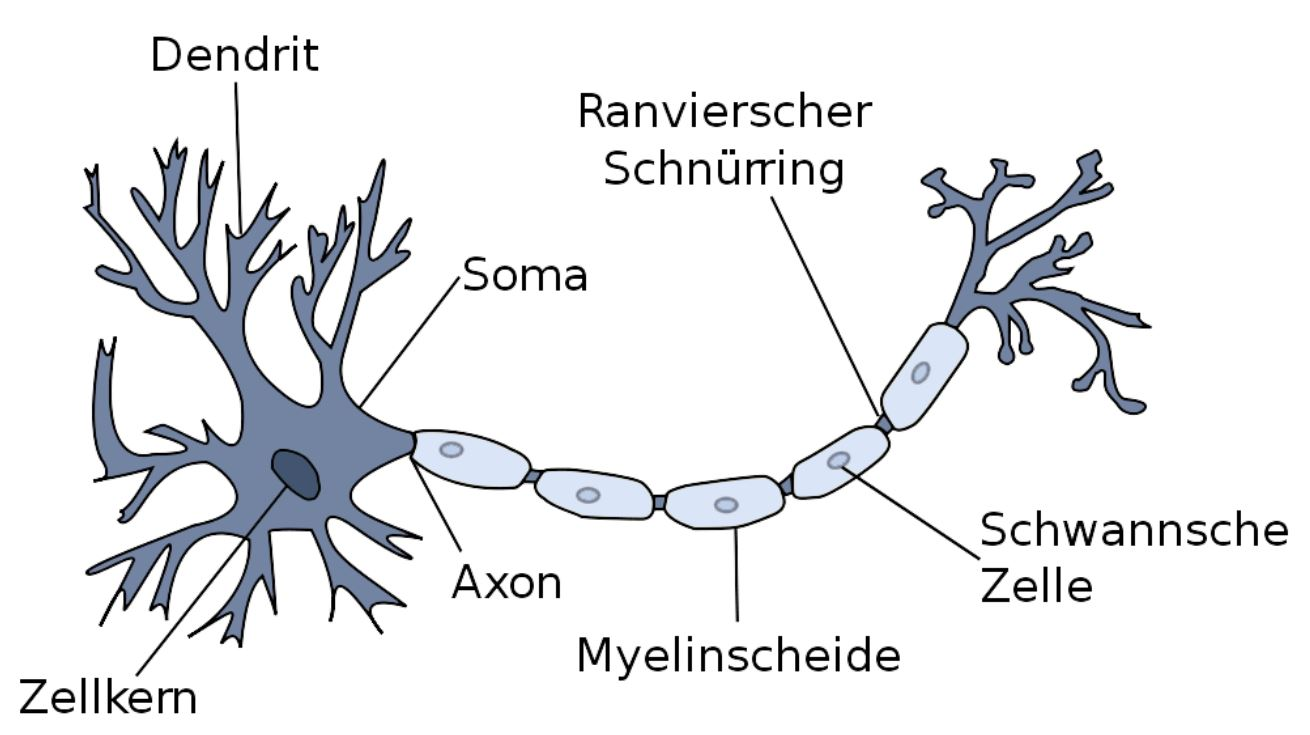
\includegraphics[width=0.75\textwidth]{./img/biologial_neuron.JPG} 
	\caption{Schematische Abbildung einer Nervenzelle, Quelle \cite{kriesel2008kleiner}.}
	\label{fig:biological_neuron}
\end{figure}
Das menschliche Gehirn besitzt ungefähr ${10}^{11}$ einzelne Neuronen, deren schematischer Aufbau in \autoref{fig:biological_neuron} dargestellt ist. Jedes Neuron besitzt einen Zellkern, der sich im Zellkörper (Soma) befindet. Von dem Zellkörper gehen mehrere Fasern aus, die Dendriten genannt werden \cite{russell2013kunstliche}. An diesen befinden sich Synapsen, welche als Übertragungsstelle fungieren und elektrische oder chemische Signale von Rezeptoren oder anderen Neuronen empfangen \cite{kriesel2008kleiner}. \\
Synapsen, die elektrische Signale empfangen, haben eine starke, direkte, nicht regulierbare Verbindung vom Sender zum Empfänger. Diese sind für hart kodierte Verhaltensmechanismen nützlich wie zum Beispiel den Fluchtreflex. Die chemische Synapse hingegen ist nicht direkt mit dem Sender verbunden, sondern durch den synaptischen Spalt getrennt \cite{kriesel2008kleiner}. Zur Übertragung eines elektrischen Signals wird dieses auf der präsynaptischen Seite in ein chemisches Signal kodiert, indem Neutransmitter freigesetzt werden. Diese können über den synaptischen Spalt übertragen und anschließend auf der postsynaptischen Seite wieder in ein elektrisches Signal kodiert werden. Ein großer Vorteil dieser Übertragungsart ist die Regulierbarkeit \cite{kriesel2008kleiner}. Verschiedene Neurotransmitter können unterschiedliche Effekte auf das Neuron haben, beispielsweise anregend (exzitatorisch) oder hemmend (inhibitorisch) sein \cite{kirschbaum2008biopsychologie}. Zusätzlich kann die Menge der freigesetzten Neurotransmitter die Stärke des Signals beeinflussen \cite{kriesel2008kleiner}. Auf lange Zeit gesehen können neue Verbindungen entstehen oder alte aufgelöst werden, was als Grundlage des Lernens im menschlichen Gehirn angenommen wird \cite{russell2013kunstliche}.\\
Sowohl die erregenden als auch hemmenden Signale werden über die Dendriten an den Axonhügel weitergeleitet, welcher sich zwischen dem Soma und dem Axon befindet. Dort werden die Signale akkumuliert. Wird bei diesem Vorgang ein gewisser Schwellwert überschritten, wird ein elektrischer Impuls erzeugt der über das Axon weitergeleitet wird \cite{kirschbaum2008biopsychologie}. Das Axon ist typischerweise 1cm in Ausnahmen sogar bis zu einem 1m lang und von der Myelinscheide umgeben, die unter anderem Schutz vor mechanischer Überanspruchung bietet \cite{russell2013kunstliche}. Zusammen mit den Ranvierschen Schnürringen  ermöglicht diese zudem eine schnellere Weiterleitung des Aktionspotenzials \cite{kirschbaum2008biopsychologie}. Das Axon endet mit dem sogenannten Endknopf oder auch Axonterminal genannt. Dieses ist mit den Synapsen von anderen Neuronen verbunden und kann beim Eintreffen eines Signals die Neurotransmitter freisetzten und somit das Signal übertragen \cite{kirschbaum2008biopsychologie}. Typischerweise ist ein einzelnes Neuron mit 10 bis 100.000 anderen Neuronen verbunden \cite{russell2013kunstliche}, die alle parallel arbeiten. So entsteht ein sehr großes und leistungsfähiges neuronales Netz. 

\subsection{Das Neuron}
\subsection{Netzstrukturen}
\subsection{Optimierungsverfahren}

Das Gebiet der Künstlichen Neuronalen Netze wird bereits seit 1943 erforscht